\documentclass[conference]{IEEEtran}
\usepackage{blindtext, graphicx}
\usepackage[utf8]{inputenc}

% Citation
\usepackage{cite}

% Graphics
\usepackage{graphicx}
\graphicspath{{images/}}
\usepackage{subfigure}
\DeclareGraphicsExtensions{.pdf,.jpeg,.png,.eps}
\usepackage{booktabs}

% Math
\usepackage[cmex10]{amsmath}

% Urls
\usepackage{url}

% Tables
\usepackage{booktabs}

% Optional packages
%\usepackage{array}
%\usepackage{mdwmath}
%\usepackage{mdwtab}
%\usepackage{eqparbox}
%\usepackage[tight,footnotesize]{subfigure}
%\usepackage[caption=false]{caption}
%\usepackage[font=footnotesize]{subfig}
%\usepackage[caption=false,font=footnotesize]{subfig}

% correct bad hyphenation here
%\hyphenation{op-tical net-works semi-conduc-tor}

\begin{document}
\title{Analysis of 2 different HEVC encoding presets for resolutions up to UHD-1}

% affiliations
\author{
\IEEEauthorblockN{Christopher Krämmer}
\IEEEauthorblockA{Institute for Media Technology\\
	TU Ilmenau\\
	Email: christopher.kraemmer@tu-ilmenau.de}
\and
\IEEEauthorblockN{Serge Molina}
\IEEEauthorblockA{ 
	Systèmes Robotiques et Interactifs\\
	UPSSITECH\\
	Email: serge.molina@kloumpt.net}
\and
\IEEEauthorblockN{Anton Schubert}
\IEEEauthorblockA{
Institute for Media Technology\\
TU Ilmenau\\
Email: anton.schubert@tu-ilmenau.de}
}

\maketitle

\begin{abstract}
Abstract
\end{abstract}

\begin{IEEEkeywords}
4k, videoquality, VMAF, bitrate ladder
\end{IEEEkeywords}

\section{Introduction}
Broader access to online media content, especially on mobile devices \cite{forecast2016cisco}, combined with an growing diversity of content has led to an increased saturation of internet backbone networks \cite{sandvine2010global}. More dynamic delivery approaches like HTTP Adaptive Streaming (\textit{HAS})\cite{seufert:2015:hassurvey} are applied to increase reliability for changing bandwidth environments, while still maintaining a high quality of experience for the consumer. This requires however, that the media content is preprocessed before delivery with video encoding and segmentation. The optimum choice of encoding parameters depends on a number of factors and is often hard to determine as generalized quality models for Adaptive Streaming are still in development \cite{raake:2017:hasqualitymodel} and not yet generally available. 

This paper aims at finding a link between predicted quality and user ratings based on the Video Multi-Method Assessment Fusion (\textit{VMAF}) metric \cite{lin2013:mmf,lin2014:fvqa} and a subjective quality experiment following ITU P.910 recommendations \cite{rec1998p}. We analyze encodings of six different 10-second sequences at varying resolutions up to \textit{UHD-1} \cite{dvb:2015:uhd1}, with three bitrates per resolution, and compare them with ratings from the perceptual test based on two different encoding presets (a "na\"{\i}ve" approach and an "expert" one).

We describe our selection of the source sequences, the encoding process and the setup for the perceptual test. As achieving reproducible results is a strong focus of this research project the preprocessing and video encoding steps have been largely automated.

Several data has been collected in addition to user ratings, such as feedback questions and rating behavior. This additional data has been collected in order to enable a deeper analysis of the subjective test results.

\section{Test Preparation}
\subsection{Video Selection}
\subsubsection{Preconsiderations}
There exists only a few public 4k video databases. They differ in content (scenario, field size, camera movement, illumination condition) as well as in technical aspects (resolution, frame rate, bit rate and color bit depth). 
To obtain reference video files for the subjective test, parts of the 4k content from the databases are used (also called source video files).
For our test we want to have a large variety between the reference video files to evoke different encoding properties. 
All the reference videos should have a duration of 10 seconds with no cuts inside.
To avoid the influence of judder, the smallest permitted frame rate of the source videos is 50 frames per second (fps). Furthermore the smallest resolution considered to be 3840x2160. If the source videos are not 4k (4096x2160 pixels) they will be upscaled before distortion. Moreover the frame rate of the reference video files is being adapted to consistent 50fps.
\newline

\subsubsection{Dataset Preparation}
For obtaining a good variety of video sequences three data bases are used: The Harmonic \cite{web:harmonic} which contains 18 different video files, Cable Labs \cite{web:cablelabs} with 9 relevant 4k contents and the Blender Foundation \cite{web:bbb} for receiving the cartoon Big Buck Bunny. They  are partial under the creative commence license and all of them are available in the ProRes format, except of Big Buck Bunny where the 4k video content can be downloaded only as a compressed video file, however there also exist high quality PNGs for all the frames of the cartoon. In order to generate a high quality reference video with the frames of Big Buck Bunny, an automatisation script is used to find a sequence with a duration of 10 seconds, to download the respective images and to encode them as a video file.
Generally, the challenge is to extract 10 seconds sequences from the original video files with no cut inside because there exists only a few.

One problem of the video sequences from the database is that even they have a high bit rate and are stored as ProRes, no conclusion referring to the contained visual quality can be done. 
For this reason a preselection with a very powerful system, able to play 4k content in ProRes with high bit rates and connected to a 4k screen, was applied.
The remaining reference videos are 6 source clips, each with a duration of 10 seconds. All the files have got a resolution of 3840x2160 pixels and are stored in the ProRes format. Because this format is a 10 bit codec only, the original color depth of each video file can not be determined.
Further specific informations about the reference videos are shown in Table \ref{tab:Specifications}.

\begin{table}[h]
	\centering
	\begin{tabular}{|l|cccc|}
		%\cline{2-6}
		\hline
		Sequence Name       & Frame Rate & Bit rate & Timestamps& Source\\
		& in fps  			& in Mbps    & m:s.ms   & \\ \hline
		Air Show            & 59.94    & 1703 & 00:48.500  &   H  \\ \hline
		Big Buck Bunny      & 60       & 2304 & 05:47.000  &   B  \\ \hline
		Fjord               & 50       & 1469 & 00:21.000  &   H  \\ \hline
		Moment of Intensity & 59.94    & 1822 & 02:16.000  &   C \\ \hline
		Snow Monkeys        & 59.94    & 1750 & 00:17.000  &   H  \\ \hline
		Streets of India    & 50       & 2094 & 00:00.000  &   H  \\ \hline
	\end{tabular}
	\caption{Meta data of the video files. The timestamps are the start positions of the extraction of 10 second sequences from the source files, where m stands for minutes, s for seconds and ms for milliseconds respectively. Further shortcuts: H = Harmonic, B = Blender Foundation, C = Cable Labs}
	\label{tab:Specifications}
\end{table}

They contain a wide range of high-level features (animation, camera motion, people, water) and low-level characteristics (brightness, contrast, texture, motion, color variance, sharpness) as can be seen in Figure \ref{fig:OverviewReferenceSequences}.

\begin{figure}[h]
	\begin{center}
		%

		\subfigure[Air Show]{%
			\label{fig:airshow}
			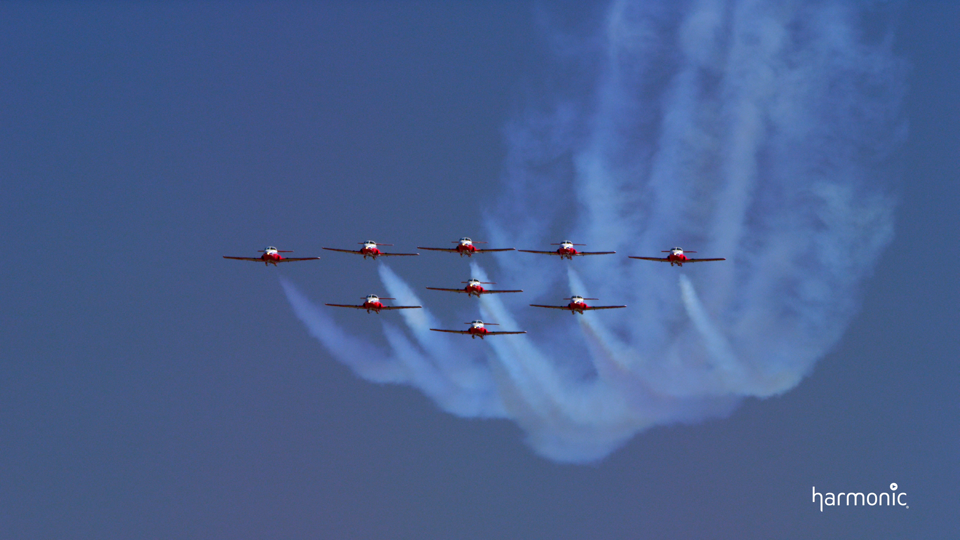
\includegraphics[width=0.2\textwidth]{images/AirShow}
		}%
		\subfigure[Big Buck Bunny]{%
			\label{fig:bbb}
			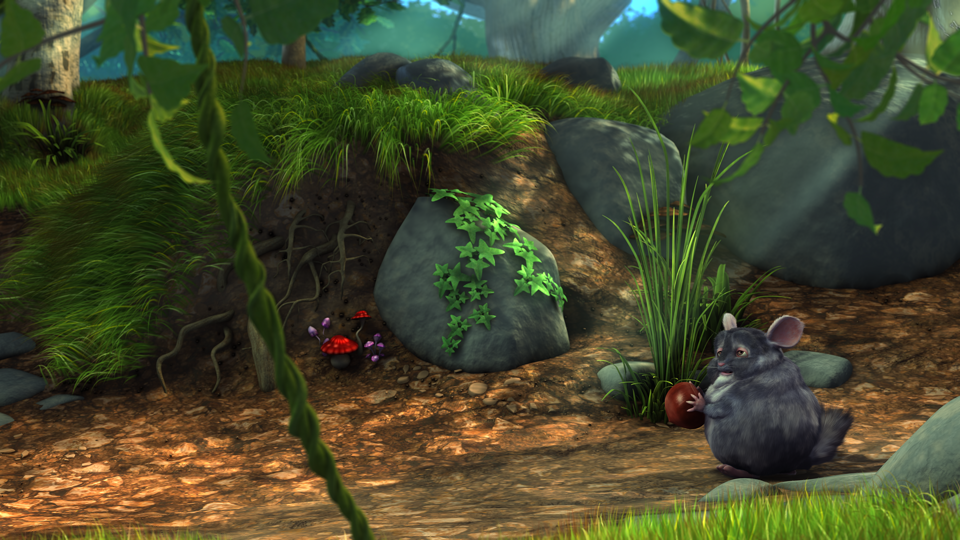
\includegraphics[width=0.2\textwidth]{images/Bbb}
		}\\ %  ------- End of the first row ----------------------%
		\subfigure[Fjord]{%
			\label{fig:Fjord}
			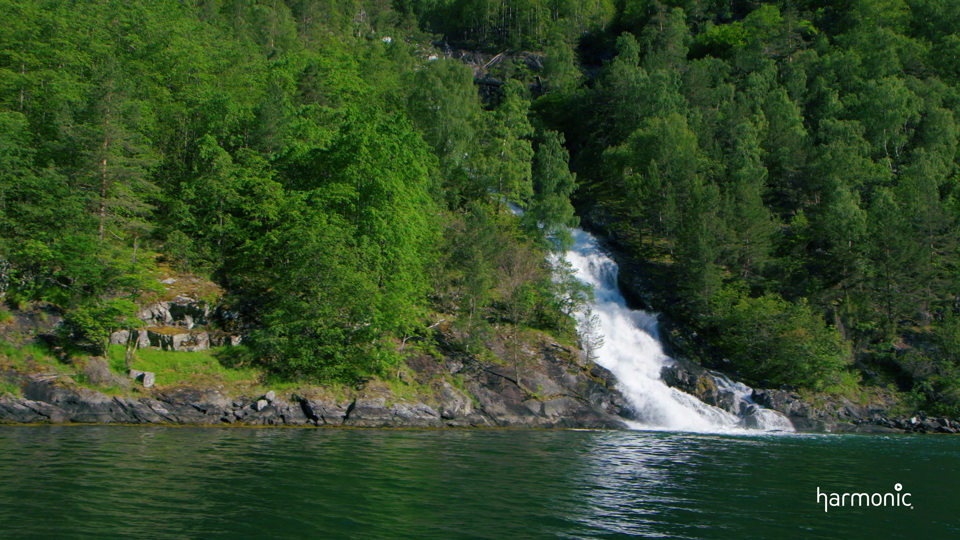
\includegraphics[width=0.2\textwidth]{images/Fjord}
		}%
		\subfigure[Moment of Intensity]{%
			\label{fig:MomentOfIntensity}
			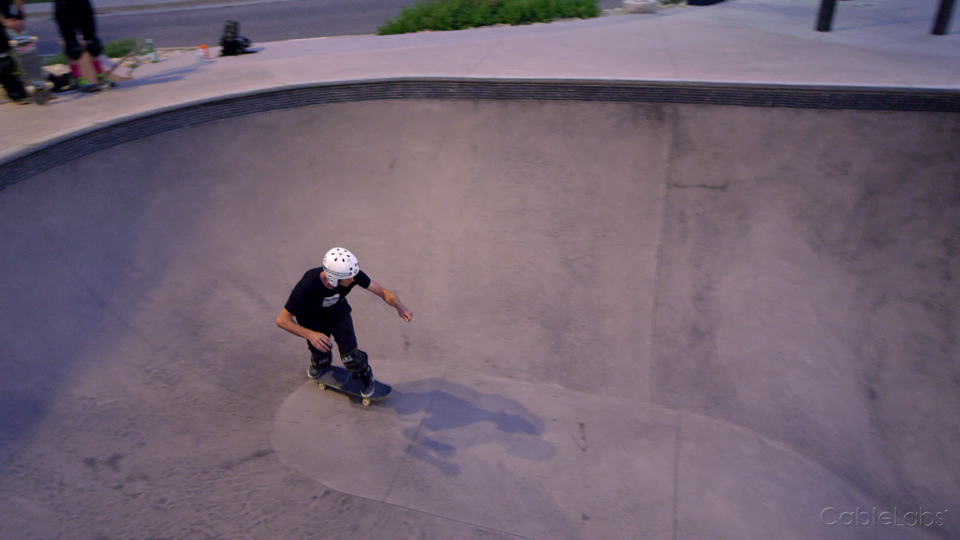
\includegraphics[width=0.2\textwidth]{images/MomentOfIntensity}
		}\\ %  ------- End of the second row ----------------------%		
		\subfigure[Snow Monkeys]{%
			\label{fig:SnowMonkeys}
			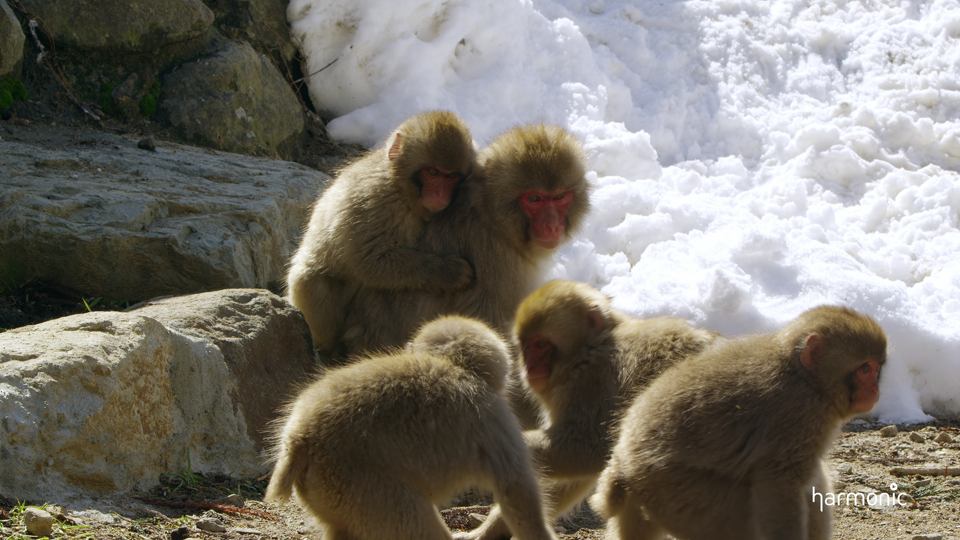
\includegraphics[width=0.2\textwidth]{images/SnowMonkeys}
		}%
		\subfigure[Streets of India]{%
			\label{fig:StreetsOfIndia}
			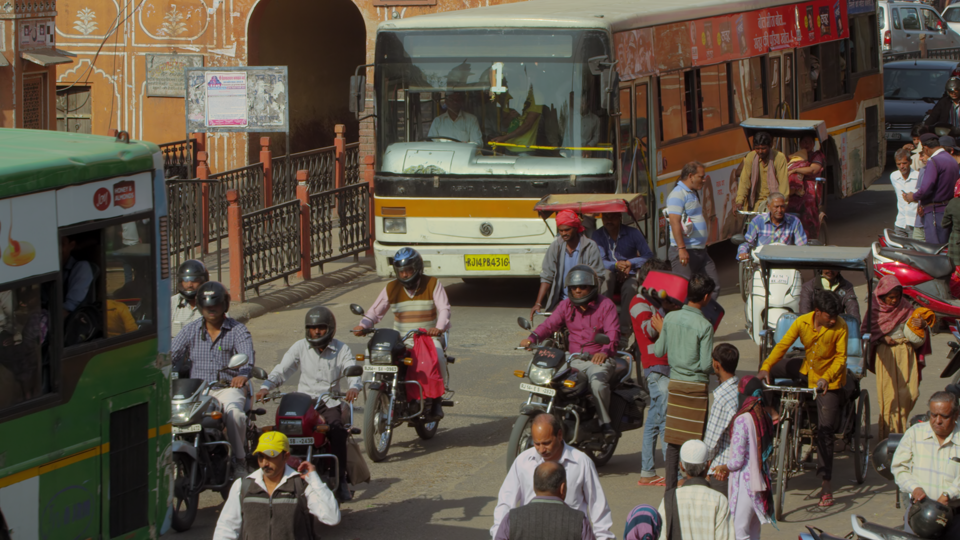
\includegraphics[width=0.2\textwidth]{images/StreetsOfIndia}
		}%
		%
	\end{center}
	\caption{%
		Selection of frames contained in the reference videos to show the variety of the content.
	}%
	\label{fig:OverviewReferenceSequences}
\end{figure}



\subsection{Encoding Parameters}
As one of the focus points of this paper the choice of encoding parameters and the video preprocessing are of main importance. This section will first cover the two different encoding presets, go over the method which is used to derive the target bitrates and finalize with a description of the process automation.

\subsubsection{Encoding Presets}
We use the open x265 encoder for our experiment as it offers good performance and integration in the FFmpeg toolchain. Two different presets are used for the sequence encodings, a "na\"{\i}ve" (1) and an "expert" preset (2). The "na\"{\i}ve" preset is a simple \textit{CBR} (Constant Bitrate) encoding, whereas the "expert" preset is a 2-pass encoding with a Quality-Control pass followed by a Bitrate-Control pass.  Every sequence is encoded with both presets at 3 resolutions (540p, 1080p, 2160p) and 3 bitrates for each resolution. The following section goes into detail on how we select those bitrates.

\begin{figure}[thb!]
	\centering
	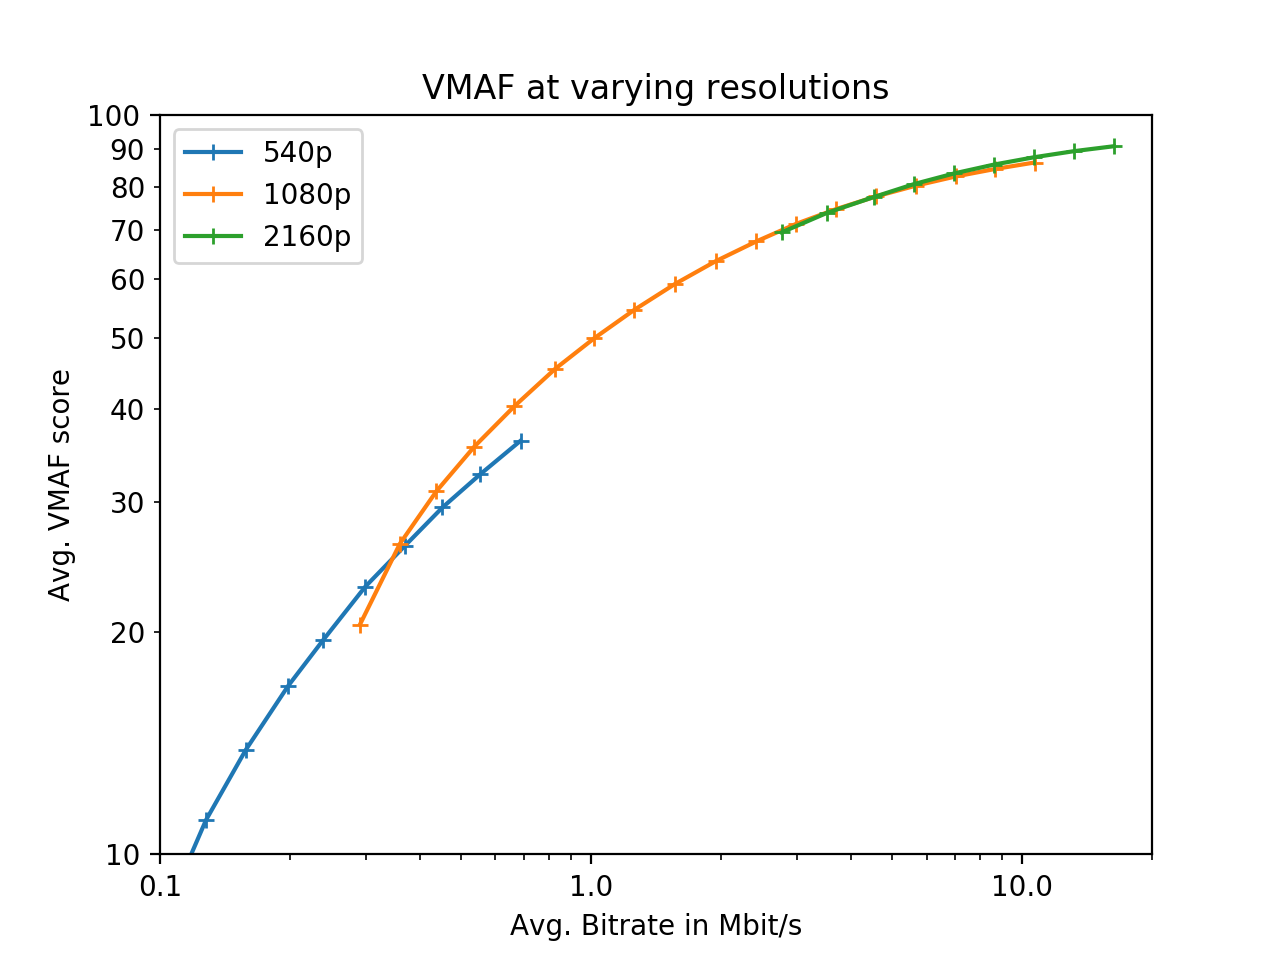
\includegraphics[width=3.5in]{vmaf_bitrates}
	\caption{Average \textit{VMAF} scores for 25 different bitrates at 3 resolutions. The encoded bitrates and the \textit{VMAF} scores are averaged between the 6 sequences and form the abscissa (Log) and ordinate respectively.}
	\label{fig:vmaf:bitrates}
\end{figure}

\subsubsection{Selection of Bitrates}
Video Multi-Method Assessment Fusion (\textit{VMAF}) is a full reference metric for estimating human perception of video quality \cite{lin2013:mmf}. We use \textit{VMAF} because it provides a better estimate of subjective quality than single metrics like \textit{SSIM} or \textit{VIF}.

To estimate relevant \textit{HEVC} encoding bitrates for our source content we sample the \textit{VMAF} scores at 25 bitrates on a logarithmic scale for our 3 different resolutions (540p, 1080p, 2160p). The reference sequences are resampled to a fixed 50 frames per seconds to avoid frame rate differences, while the distorted sequences are downsampled, encoded with \textit{CBR} rate control and upsampled to \textit{UHD-1} again using lanczos resampling. Both presets use 4:2:0 chroma subsampling to be close to the typical use-case of webvideo. The sampling requires 222 total sequences to be encoded with x265 and analyzed with the \textit{VMAF Development Kit} (VDK). This process takes around 18 hours (excluding download and cutting of the source material) on a current 10-Core x64 CPU.

The resulting \textit{VMAF} scores exhibit an overlap between different resolutions and the final encoding bitrates are chosen near those intersections. Figure \ref{fig:vmaf:bitrates} shows the sampled scores with the target rates in the background. We choose the target bitrates at least 2 bitrate-samples away from an intersection with the next quality, except for the lower 1080p-bound where it is not possible to lower the bitrate any further due to encoder restrictions. This should ensure a relevant sampling of the \textit{MOS}-bitrate space for the subjective test.

\begin{figure}[thb!]
	\centering
	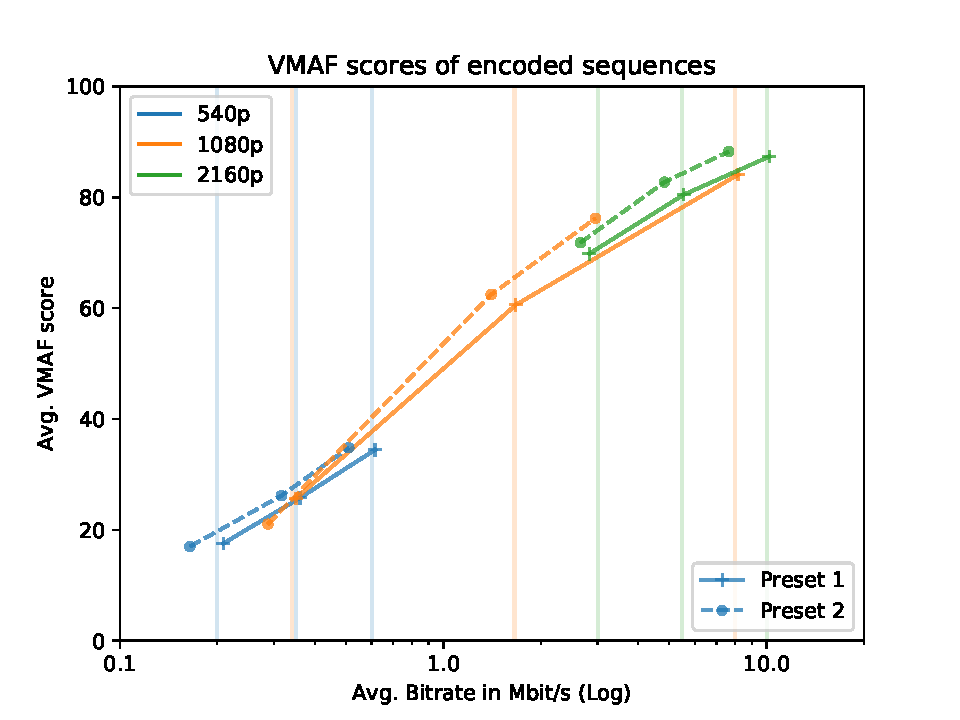
\includegraphics[width=3.5in]{vmaf_final}
	\caption{Average \textit{VMAF} scores of encoded videos for both presets. The encoded bitrates and the \textit{VMAF} scores are averaged between the 6 sequences for each preset and form the abscissa (Log) and ordinate respectively.}
	\label{fig:vmaf:encoded}
\end{figure}

The average \textit{VMAF} scores of the two presets at the chosen bitrates can be seen in Figure \ref{fig:vmaf:encoded}. The respective target bitrates can be seen in the background again. The scores of the "expert" preset (2) are consistently higher than the ones for the "na\"{\i}ve" preset (1) at matching target bitrates. Furthermore, the "expert" preset saves bitrate by resorting to an acceptable level of quality, while the "na\"{\i}ve" presets bitrates are very close to the targets. However, we can see that the preset two sometimes reduces the bitrate too far so that the average score is well below preset one. This happens especially for the lowest 1080p bitrate and less so for the 540p encodings.


\begin{figure}[bht!]
	\centering
	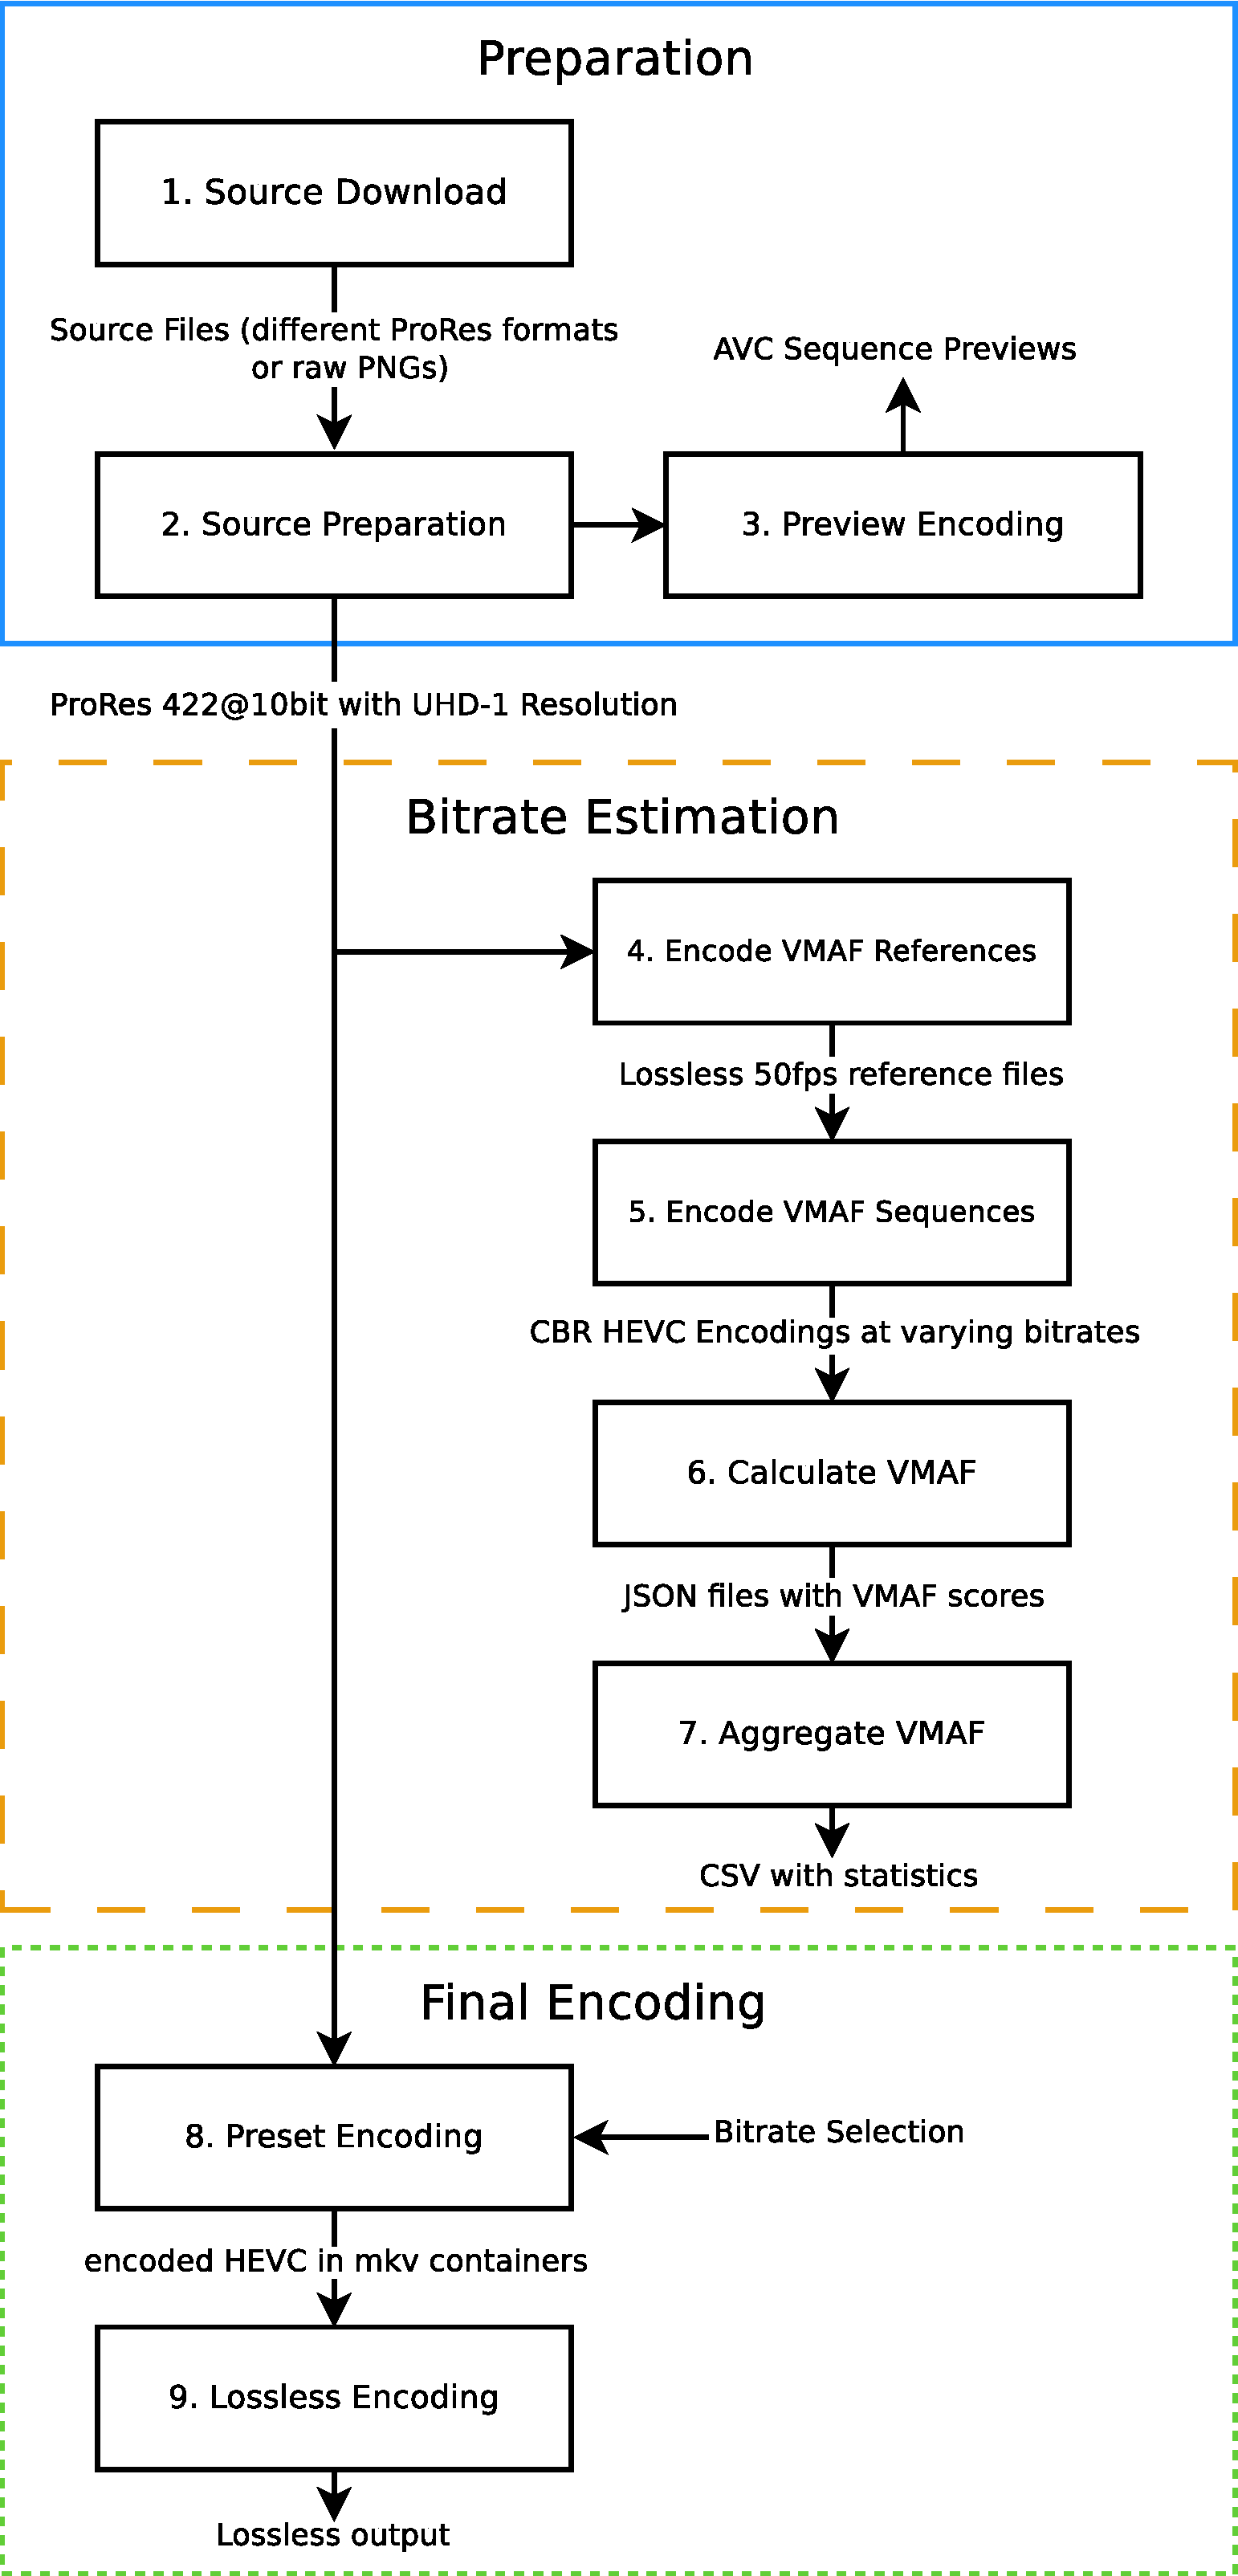
\includegraphics[width=2.5in]{automation}
	\caption{Automated processing and encoding workflow.}
	\label{fig:automation}
\end{figure}

\subsubsection{Encoding Automation}
We automate the whole process for downloading, preprocessing and encoding the source videos using pydoit \cite{web:pydoit}. This speeds up the turnaround time for changed parameters or sequences and also ensures that the encoded material can later be reproduced.

The whole process is illustrated in Figure \ref{fig:automation} and starts with the source preparation (A). After download of the sequences (1) they are cut to 10 seconds length and saved as ProRes HQ with \textit{UHD-1} resolution (2). Additionally, \textit{MPEG4-AVC} previews are generated at a lower resolution of 1440p to allow review of the sequences on slower devices.

After the initial processing the bitrate estimation is performed (B) using the \textit{VMAF} metric \cite{lin2013:mmf}. The videos are brought to the same frame rate of 50fps (4) and encoded with \textit{CBR} at 25 different bitrates (5). The average \textit{VMAF} score of each video is analyzed with the \textit{VMAF} Development Kit (VDK) \cite{web:vdk} and saved as a json file (6). All of the average scores are then aggregated into a single CSV for plotting and further analysis (7). The target bitrates can then derived from these scores.

The last step is the main encoding (C). It can only start after the target bitrates have been specified in the configuration. The sequences are encoded first with the two presets (8) and transcoded to a lossless format (ffvhuff) afterwards, to allow for fast and consistent playback as well as archiving of the video material.




\subsection{Test Setup}
Several steps have been followed in order to enable the acquisition of meaningful data during the subjective tests. Theses steps included defining the test environment, choosing a rating framework and creating additional question that may help inferring informations about the participants and their way of rating content.

\subsubsection{Test Environment}
In order to make the results of our research reproducible the ITU P.910 recommendation \cite{rec1998p} have been followed. 
The parameters include aspects such as viewing distance, peak luminance of the screen or background room illumination.
As performing tests following these specifications is common at the Technical University of Ilmenau, a room meeting these requirements was available and therefore used.
The specifications of the room was the following for each of the parameters:


	
\subsubsection{Rating Framework}
The testing procedure which seems more suited to the case was Absolute Category Rating (ACR) \cite{rec1998p}, where different versions of an original sequence are shown to a test participant. 

For each sequence the participant issues categorical ratings from any of these 5 answers: \{Excellent, Good, Fair, Poor, Bad\}


The steps performed by a participants during a rating session can be seen in the figure \ref{fig:workflow:state_machine}.

\begin{figure}[h]
	\centering
	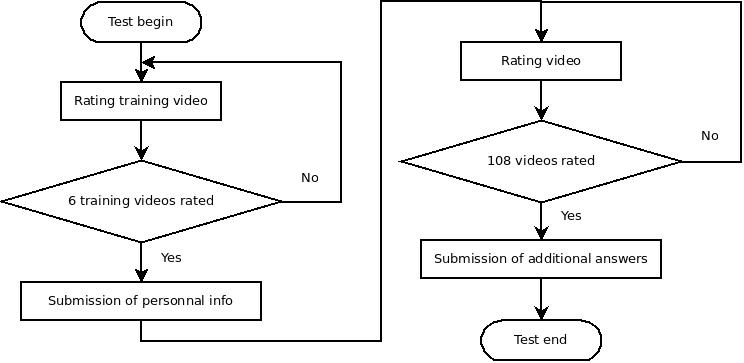
\includegraphics[width=3.5in]{rating_workflow}
	\caption{Detailed steps of the rating workflow}
	\label{fig:workflow:state_machine}
\end{figure}

\subsubsection{Additional collected data}
In order to gain more knowledge about the users behaviour, additional data is collected from the participants.

One of the suggestions of the ITU recommendation paper being the usage of several test questions in addition to the ratings \cite{rec1998p}, the following questions have been asked at the end of each rating session:

\begin{itemize}
	\item Presence of blocky artefacts
	\item Visible bands of colour
	\item Smoothness of the playback
	\item Have you seen 4K content before?
	\item Have you seen content on a 4k screen before?
	\item How sure were you about the rating that you provided?
\end{itemize}




These idea behind these question is dual as these questions may translate how users percieve/are sensitive to video features as well as how users may clearly express their perceptions. As it has already been noticed in previous experiments and in discussions with test participants: users may still rate using a different scales, thus spreading the final MOS or falsely being classified as outlier when their ratings may only represent a shift from the overall population. 

Moreover, mouse interactions have been collected during the rating of each sequence. The intent behind this is that as the MOS scale doesn't allow detailed answers some participants may hesitate between two answers and change their answers or hover with their mouse around some answers. Also, answering speed, which could be an indicator of a participant skipping answers or to the contrary being strongly confident of his answers. We believe that several informations can be extracted from these kind of behaviours:
\begin{itemize}
	\item Confidence in the participant sequence rating
	\item Confidence in the participant overall rating
	\item Intermediate scores (eg: 4.5)
\end{itemize}


\section{Test Results}
\subsection{Ratings}
(MOS Results, Plots and stuff)

Pure result numbers here only, analysis in evaluation

\textbf{Compare preset MOS}

\begin{figure*}[t!]
	\centering
	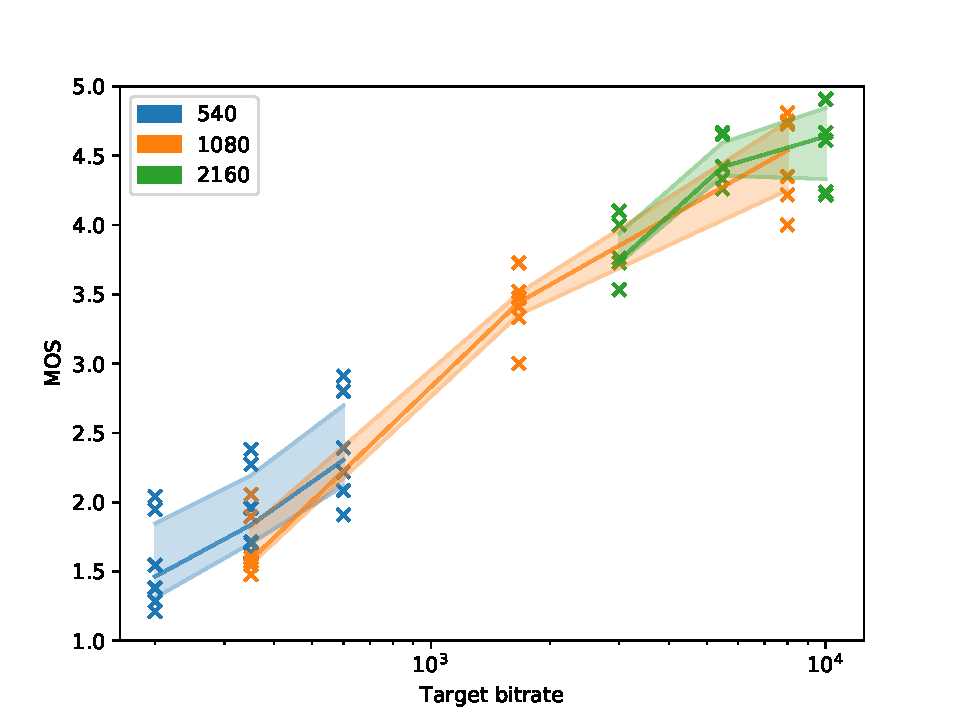
\includegraphics[width=3.5in]{correlation_bitrate_mos_p1}
	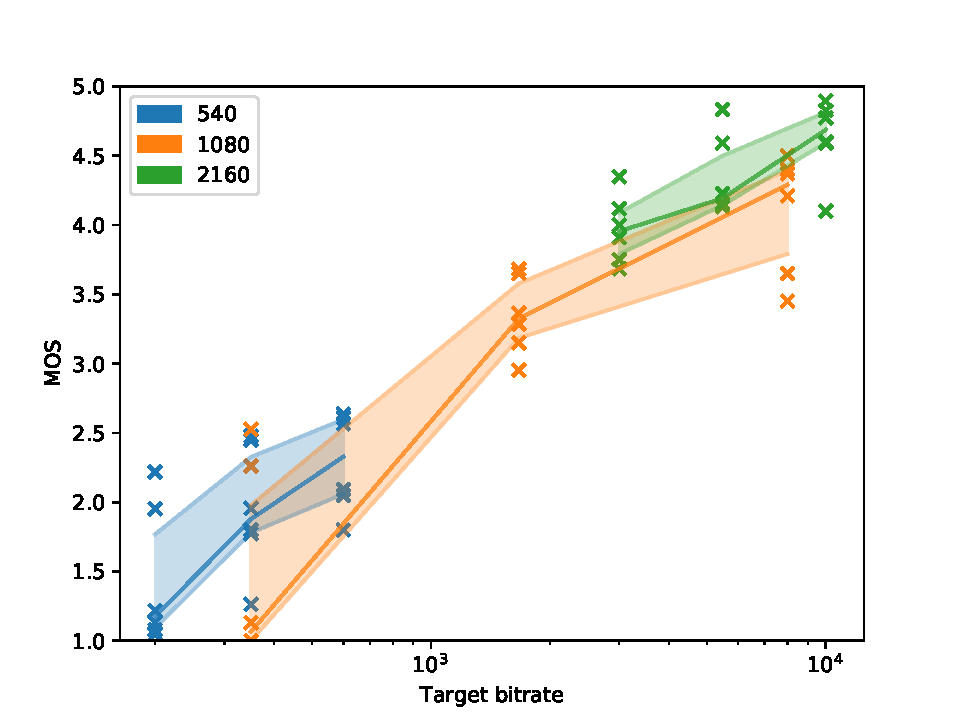
\includegraphics[width=3.5in]{correlation_bitrate_mos_p2}
	\caption{Correlation between bitrate and MOS for both encoding presets. The center line represents a median and the outer line the 25th and 75th percentile of MOS for the 6 sequences.}
	\label{fig:result:correlation_bitrate_mos}
\end{figure*}

The Distribution of MOS values for each preset at different resolutions is shown in Figure \ref{fig:result:correlation_bitrate_mos}.

The "expert" preset is not using all available bitrate in critical low-bitrate situations. (Drop-Off for 1080p MOS), can already be predicted from VMAF plot.


\textbf{Participant outliers}
\begin{figure}[bht!]
	\centering
	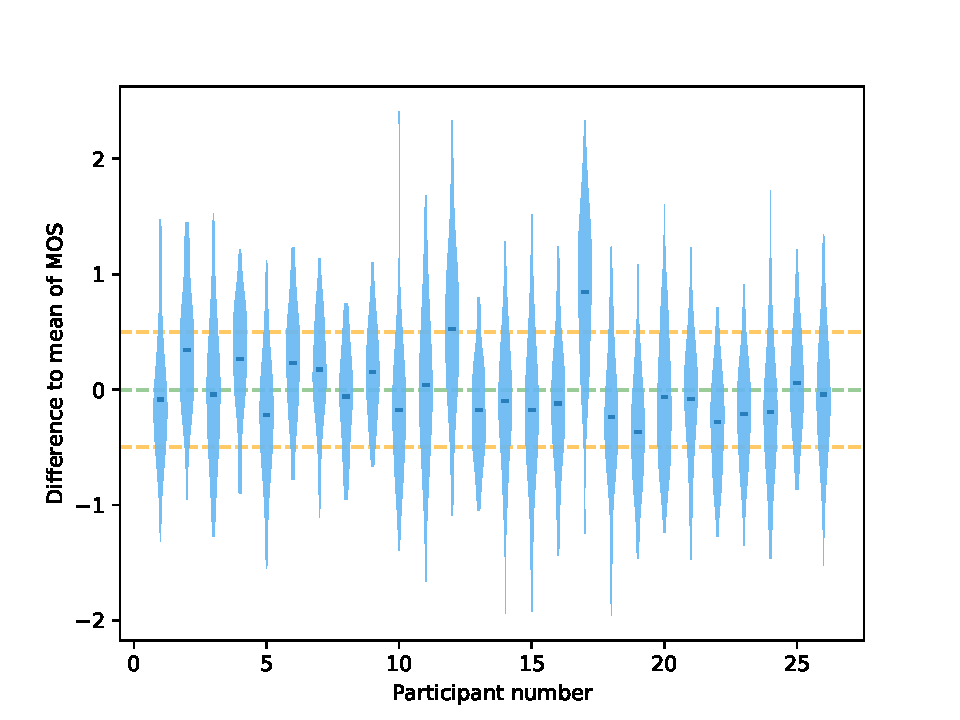
\includegraphics[width=3.5in]{participant_mos_violin}
	\caption{}
	\label{fig:result:participant_violin}
\end{figure}
\\

\textbf{Compare MOS with vmaf (correlation?)}
\begin{figure}[bht!]
	\centering
	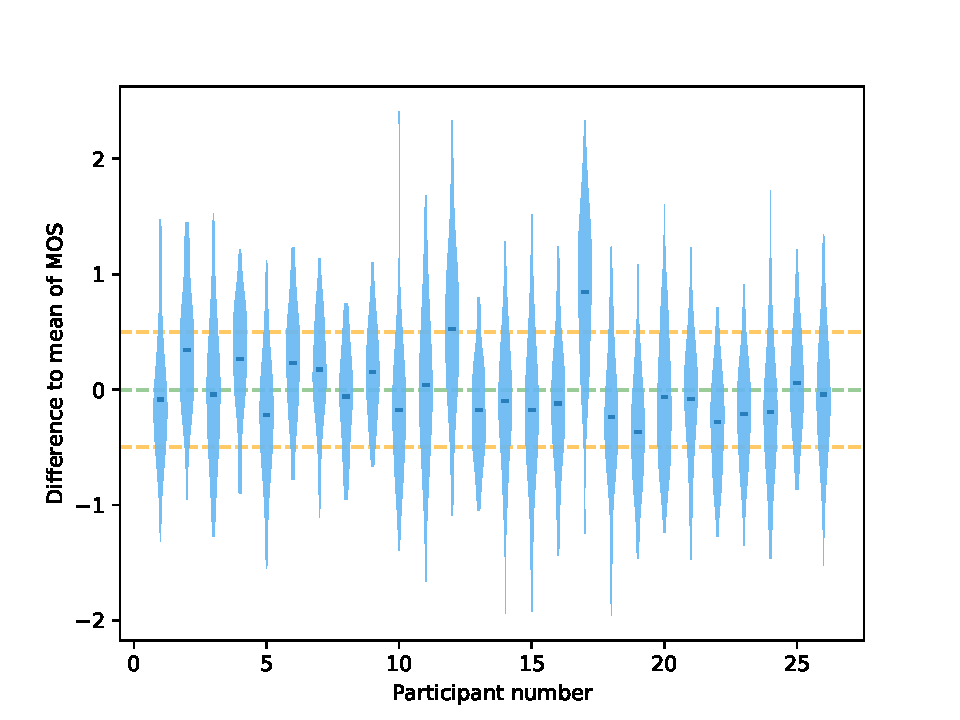
\includegraphics[width=3.5in]{participant_mos_violin}
	\caption{}
	\label{fig:result:participant_violin}
\end{figure}
\\

\textbf{Bitrate savings}
\begin{figure}[bht!]
	\centering
	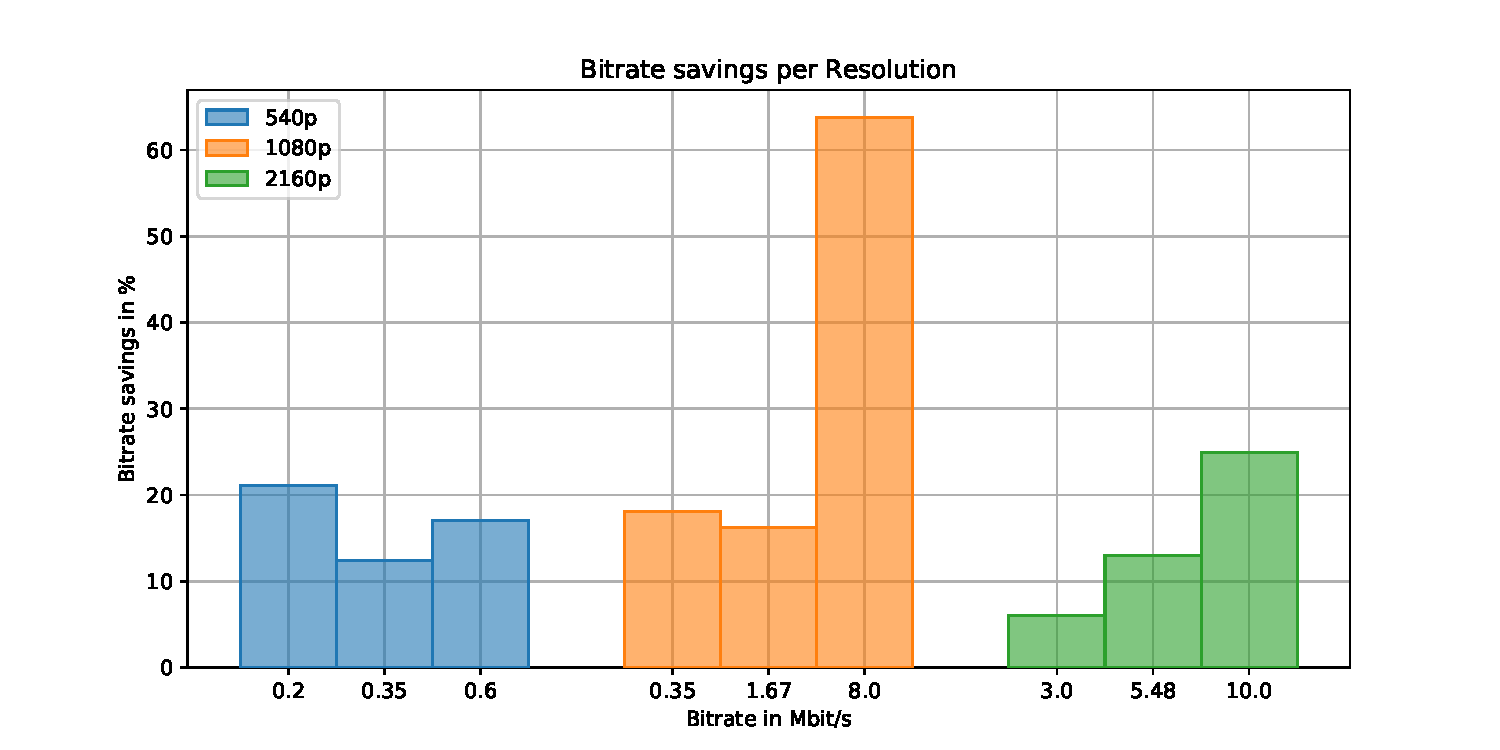
\includegraphics[width=3.5in]{bitrate_savings}
	\caption{}
	\label{fig:result:bitrate_savings}
\end{figure}
\begin{figure}[bht!]
	\centering
	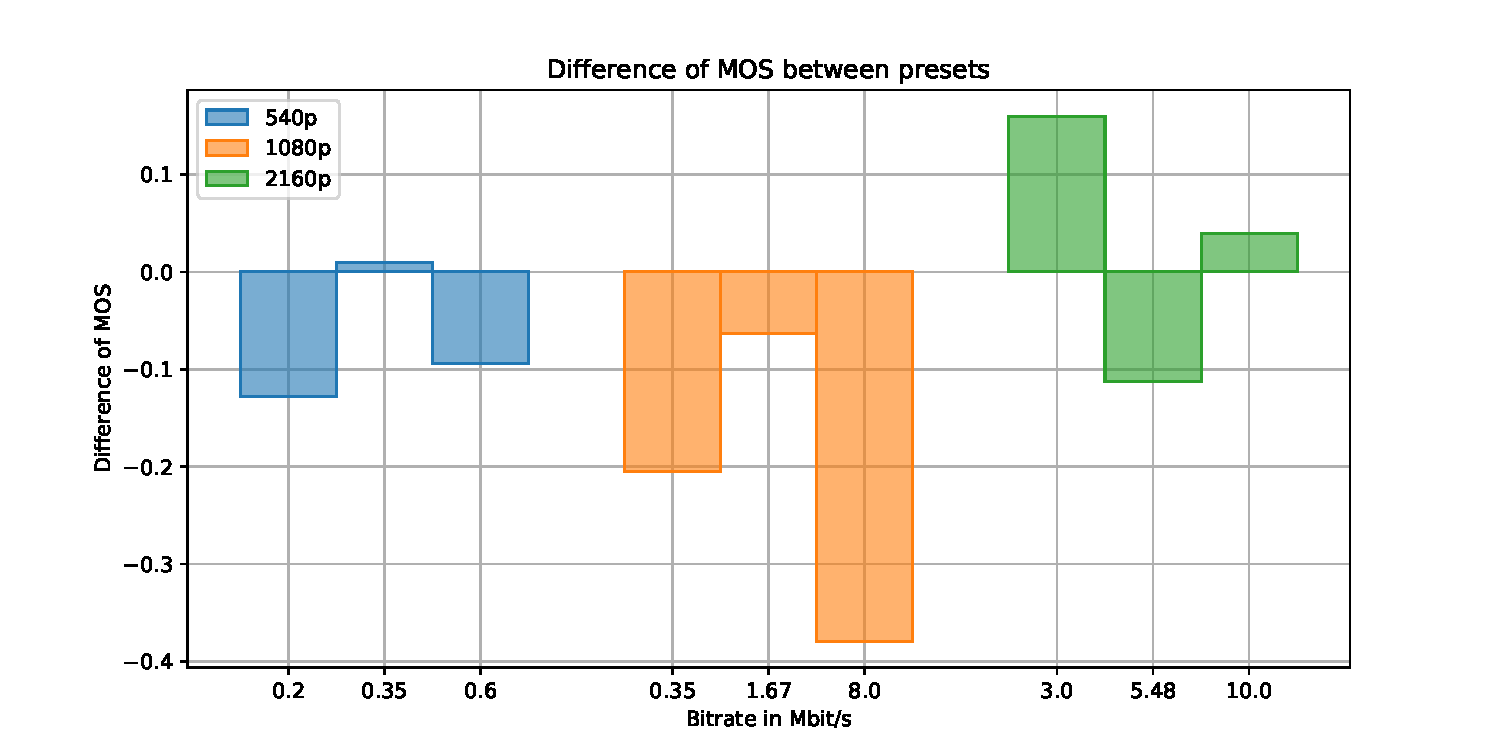
\includegraphics[width=3.5in]{quality_difference}
	\caption{}
	\label{fig:result:quality_difference}
\end{figure}

\subsection{Features}
Correlation between answers to the feedback questions and the ratings values and characteristics have been computed. These correlations were not significant enough to be further analysed. Although mouse movements was collected, it has not been analysed.

\section{Conclusion}
\subsubsection{Conclusion}
The final subjective quality can be accurately predicted using the \textit{VMAF} metric.
Our aggressive optimization approach with the "expert" encoding preset pays off at higher bitrates but degrades visual quality for low bitrates. This suggests that high-effort multi-pass encodings mainly benefit high resolution content at large bitrates, where the absolute gain can also be larger.


\subsubsection{Future Work}
Improvements of the automation framework: The source Preparation step could directly transcode the original material to a constant framerate and color-subsampling in a lossless format to avoid a further preprocessing step for the VMAF metrics.

A longer test or a sectioned test with more participants would provide a better sampling of the bitrate-MOS space and allow for more detailed analysis.

The test could be done to specifically look at content-specific encoding approaches like \cite{cock:2016:titleencode}.



%\appendices
%\section{Proof of the First Zonklar Equation}

% use section* for acknowledgement
%\section*{Acknowledgment}
%The authors would like to thank...

% trigger a \newpage just before the given reference
% number - used to balance the columns on the last page
% adjust value as needed - may need to be readjusted if
% the document is modified later
%\IEEEtriggeratref{8}
% The "triggered" command can be changed if desired:
%\IEEEtriggercmd{\enlargethispage{-5in}}

% References
\bibliographystyle{IEEEtran}
\bibliography{IEEEabrv,paper}

\end{document}


